% This version of CVPR template is provided by Ming-Ming Cheng.
% Please leave an issue if you found a bug:
% https://github.com/MCG-NKU/CVPR_Template.

%\documentclass[review]{cvpr}
\documentclass[final]{cvpr}

\usepackage{times}
\usepackage{epsfig}
\usepackage{graphicx}
\usepackage{amsmath}
\usepackage{amssymb}

% Include other packages here, before hyperref.

% If you comment hyperref and then uncomment it, you should delete
% egpaper.aux before re-running latex.  (Or just hit 'q' on the first latex
% run, let it finish, and you should be clear).
\usepackage[pagebackref=true,breaklinks=true,colorlinks,bookmarks=false]{hyperref}


\def\cvprPaperID{****} % *** Enter the CVPR Paper ID here
\def\confYear{CVDL 2021}
\setcounter{page}{1} % For final version only


\begin{document}

%%%%%%%%% TITLE
\title{RepVGG: Making VGG-style ConvNets Great Again}

\author{Felix Hausberger\\
	Universität Heidelberg\\
	Grabengasse 1, 69117 Heidelberg\\
	{\tt\small eb260@stud.uni-heidelberg.de}
}

\maketitle

%%%%%%%%% ABSTRACT
\begin{abstract}
	
\end{abstract}

%%%%%%%%% BODY TEXT

% Introduction
\section{Introduction} \label{introduction}
% Problem statement, motivation, main idea

VGG\footnote{Visual Geometry Group, Department of Engineering Science, University of Oxford} \cite{KarenSimonyan.2014}, Inception \cite{ChristianSzegedy.2014}, ResNet \cite{KaimingHe.2015}, DenseNet \cite{GaoHuang.2016}, Xception \cite{FrancoisChollet.2017}, ResNeXt \cite{SainingXie.2017}, EfficientNet \cite{LeMingxingTan.2019}, RegNet \cite{IlijaRadosavovic.2020}, the history of research in convolutional neural networks (CNNs) is an ancient discipline in computer vision. Over the years such CNNs became more and more accurate and efficient, but also more complicated to implement and to understand as many architecture-specific ideas and components got introduced. Such architectures do not even need to be manually designed anymore as neural architecture search (NAS) methods give the opportunity to learn optimal architectural designs right away. Old VGG-style plain CNNs containing only 3x3 convolutional, pooling and ReLU activation layers seem to be almost completely out-of-date. 

Besides all the benefits of enabling the training of deeper and more accurate models such architectures also have a few downsides. Multi-branch models are not only difficult to implement and to customize, they also do not manage to achieve a decent speed-accuracy trade-off anymore as the multi-branch architectures introduce high memory access costs (MACs) by branch additions/concatenations, depthwise separable convolutions or channel shuffling (see \autoref{related_work}). A further factor for reduced inference speed are the synchronization overheads through the many distinct architectural components (especially in NAS-created models) which make parallelism more difficult. Plain VGG-style models do not own such inherent speed bottlenecks and high memory costs, also they are not bound to certain constraints like shape matching needed for branch additions and are also more friendly to channel pruning \cite{HaoLi.2017} which removes low-impact filters. On the other hand, plain VGG-style models are difficult to train to decent depths because of vanishing gradient problems. They also cannot be used as an implicit ensemble of multiple shallower models as ResNet-like architectures can. 

RepVGG therefore introduces a re-parameterization method that helps to transform parameters of a ResNet-like training-time architecture to a VGG-like inference-time architecture using simple linear algebra. The resulting model can thus be trained until reasonable accuracy by the increased depth and an implicit ensemble-like setup during training and still achieves far higher speed during inference compared to current multi-branch models. The few types of operators needed for the VGG-like inference-time architecture and its single branch character also help to integrate more computing units onto the chip, which can furthermore individually be optimized on hardware-level giving additional speed gains. Having a plain feed-forward architecture during inference also makes the final model more memory-efficient in the end. 

The goal of RepVGG is it therefore to provide a simple and efficient VGG-style plain CNN during inference obtained by applying a structural re-parameterization onto a trained ResNet-like multi-branch model. RepVGG will be evaluated both for image classification on ImageNet \cite{JiaDeng.2009} as well as for semantic segmentation on Cityscapes \cite{MariusCordts.2016}. 

Before the re-parameterization method and architecture of RepVGG will be introduced, an extensive examination of the fundamentals and related work will be given. Many of the models introduced in this section will be important for major arguments, comparisons and the context of later parts of this paper. 

%-------------------------------------------------------------------------

% Fundamentals and related work
\section{Related Work}

The VGG architecture was introduced in \cite{KarenSimonyan.2014}. One of its key finings was to prefer deep CNNs (16-19 weight layers) with small receptive fields induced by using small kernels over shallow CNNs with bigger receptive fields. Therefore a configuration of 3x3 kernels with stride 1 were used. This not only helps to strengthen the discriminative character of the network as the non-linear activation function (ReLU) is applied more often but also keeps the number of parameters to train lower. To increase the non-linearity without affecting the related receptive fields even 1x1 kernels were considered in more deeper architectures. Only by using simple convolutional, max-pooling and fully connected layers at the end of the network, VGG achieved a 24.4 top-1 validation error score during ILSVRC-2014 (single net performance). \cite{KarenSimonyan.2014}

Regarding the top-5 test error score VGG got beaten by GoogLeNet with 6.67 compared to 7.32 from VGG. GoogLeNet uses a very deep CNN with 22 trainable layers with nine of them being the novel inception modules. To counter the higher computational costs that come with deeper architectures and also to prevent overfitting when having a limited dataset, an inception module uses 1x1 kernels for dimension reduction and to also detect cross-channel correlations. To better recognize spatial correlations and objects at various scales, an inception modules applies 1x1, 3x3 and 5x5 kernels simultaniously and bundles its results for the next layer making the network architecture also wider than others. \cite{ChristianSzegedy.2014}

When trying to answer the question how deep CNNs can get the so-called degradation problem was discovered. During training it was experienced that the loss curve started to ascent again once a specific depth threshold was passed. This was because once an ideal mapping to the right output vector was learned up until a certain depth by shallow layers, it was difficult to train the remaining layers to keep these values by learning an implicit identity function through several non-linearity steps. ResNet solved the degradation problem by introducing so-called \textit{shortcut connections} that forward intermediate network values to deeper layers. The skipped network layers therefore only needed to learn the residual towards the expected output values giving ResNet its name. Therefore in case the optimal output is already learned, the weights of a residual component will turn to zero and an identity function is realized. Training an ensemble of 152 layer-deep ResNets on ImageNet as part of the ILSVRC-2015 challenge resulted in a 3.57 top-5 test error score beating both VGG and Inception from the previous challenge while keeping complexity eight times lower than VGG for a single net. \cite{KaimingHe.2015}

The shortcut connections introduce different paths through the network rather than having one single deep network feed-forward flow. Later studies of residual architectures found out, that these paths do not necessarily depend on each other although being trained jointly. Even further, those paths that contribute the most to the gradient flow rather represent an ensemble behavior as the performance smoothly correlates with the number of valid paths. These valid paths make up only 0.45\% of all paths and are predominantly short paths through the network whereas deep paths do not contribute any gradient. Those findings were proven experimentally by changing the structure of a residual network without having impacted its performance, removing residual modules mostly impacts long paths that don't contribute to the gradient flow. \cite{AndreasVeit.2016}

The Inception architecture was lateron combined with the new residual connections idea from ResNet forming the revised Inception-ResNet architecture \cite{ChristianSzegedy.2016}.

The journey continues with DenseNet, a novel network architecture that feeds a layer all outputs from previous layers and passes its own feature maps towards all consecutive layers inside so-called dense blocks. It therefore makes feature propagation stronger by making feature reuse possible. Compared to ResNet, DenseNet achieves a lower error rate on CIFAR-10 with 4.51 to 6.61 at comparable depth while having less parameters to train. \cite{GaoHuang.2016}

A groundbreaking achievement was published with EfficientNets, a series of network architectures that were uniformly scaled in depth, width and resolution using a compound scaling method with fixed scaling coefficients for different hardware memory limits. 

\begin{figure}[t]
	\begin{center}
		% \fbox{\rule{0pt}{2in}\rule{0.9\linewidth}{0pt}}
		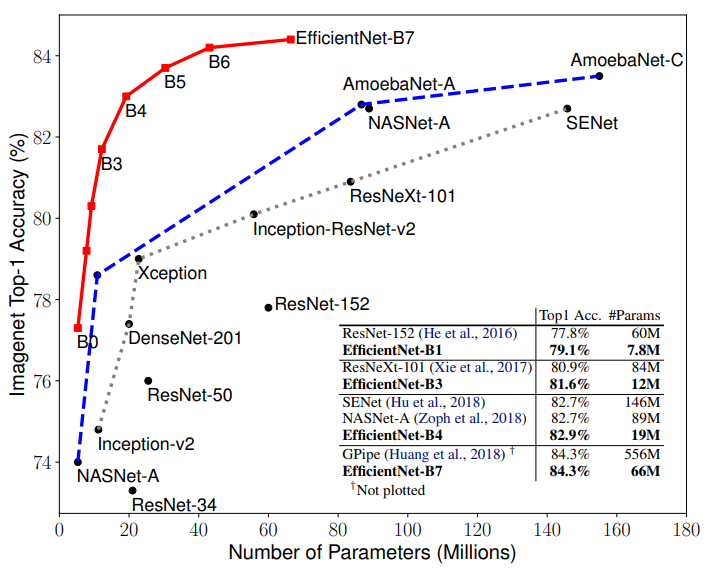
\includegraphics[width=0.8\linewidth]{images/efficientnet.PNG}
	\end{center}
	\caption{Comparison of EfficientNet to other state-of-the-art architectures on ImageNet (top-1 accuracy) compared to the number of parameters used}
	\label{fig:efficientnet}
\end{figure}

\autoref{fig:efficientnet} shows a 84.3\% top-1 accuracy score of EfficientNet-B7 on ImageNet outperforming other networks like ResNet or DenseNet while at the same time having far fewer parameters to train. \cite{LeMingxingTan.2019}

All these recent achievements on CNNs were based on manual architecture search. As opposed to such manual search, neural architecture search (NAS) tries to automate the process of finding suitable network architectures by applying a policy-gradient based reinforcement learning method over a specified design space. A RNN therefore continuously creates new network architectures which get evaluated on a target dataset. The achieved accuracy is then fed back as a reward signal to the RNN. \cite{LeBarretZoph.2017}

In \cite{BarretZoph.2018} this NAS is first performed on the small CIFAR-10 dataset in order to efficiently find a suitable architecture for a single convolutional cell. The design space used is called NASNet. The resulting cell architecture is then stacked to an entire CNN to perform image classification on the larger ImageNet dataset. Each convolutional cell has the same architecture but different weights. NASNet achieves a 2.4\% error rate on CIFAR-10 and a 82.7\% top-1 accuracy, resp. 96.2\% top-5 accuracy on ImageNet while having 28\% less computational complexity. 

This method was lateron outperformed by \cite{ChenxiLiu.2018} which uses a heuristic search to find suitable convolutional cells and a surrogate function to predict its performance to limit the amount of convolutional cells to train. It is five times more efficient regarding the number of models evaluated and eight times faster regarding the total computational effort than \cite{BarretZoph.2018}. 

Besides reinforcement learning methods there is also an evolutionary algorithms approach to neural architecture search with comparable results in model accuracy \cite{EstebanReal.2019}.

One layer of abstraction higher, one can also search for suitable design spaces in order to derive a common understanding about important design principles. RegNet is such a design space derived from AnyNet, the largest possible design space without further constraints, by iteratively parametrizing whole populations of diverse networks and searching for the simplest but most perfomant population. Using this technique one can iteratively eliminate design space dimensions that are actually not too important for the network design because of similar perfomances. For instance, using a bootleneck compression ratio does not influence model performance and could thus be excluded from the design space by making it a static constraint. Increasing the depth or width of networks on the other hand is one of the key design space dimensions. The resulting population of RegNet was able to outperform EfficientNet. \cite{IlijaRadosavovic.2020}

There are some other achitecture worth mentioning, one of them being Xception. It uses so-called depthwise separable convolutional layers, which are similar to the  multi-branch architectural Inception componenets from GooLeNet, but first convolutes spatially and afterwards convolutes the resulting channels using 1x1 convolutional layers (pointwise convolution) without using non-linearity components in between. It therefore maps spatial and cross-channel correlations completely separately. The Xception architecture is a linear stack of depthwise separable convolution layers with residual connections, but only achieves negligible improvements on its competitor Inceptionv3 on ImageNet. \cite{FrancoisChollet.2017}

MobileNet takes use of such depthwise separable convolutional layers in their nature of data reduction in order to make CNNs accessible for mobile and embedded systems. It furthermore introduces two more hyperparameters, a width multiplier and resolution multiplier, to better trade-off between speed and accuracy (respectively latency and size). The width multiplier is multiplied with the input and output channels of each layer thus reducing the computational costs and number of parameters quadratically. Same goes for the resolution multiplier that is applied to the input image and subsequent layers. 95\% of the computation time and 75\% of the parameters of such MobileNets can be traced back to the pointwise 1x1 convolutions. In terms of accuracy MobileNet can be compared to VGG16 while being 32 times smaller and 27 times less computationally expensive (measured by the Mult Adds). \cite{AndrewGHoward.2017}

ShuffleNet designed for mobile devices also builds upon depthwise separable convolutional layers and combines it with pointwise group convolution to gain additional speed through reducing computational expenses in a novel way. Possible information bottlenecks by the pointwise group convolution are tackled by using subsequent channel shuffeling to keep the information flow entropy of channels the same. ShuffleNet outperforms MobileNet by having a 7.8\% lower ImageNet top-1 error at level of 40 MFLOPs, but also having 32 layers more than the original MobileNet. Nevertheless succeeding experiments reduced depth still showed a superior behavior. \cite{XiangyuZhang.2017}

The next evolutionary step of ShuffleNet was made compliant to several design principles derived to optimize general model behavior. Oftentimes the indirect metric of FLOPS as a measure for computational complexity is taken to derive speed quality guarantees of a network. Nevertheless, the direct metric speed is influenced by far more parameters than just FLOPS like memory access costs (MAC), the degree of parallelism and the optimized runtime of the target platform making FLOPS as a solely metric insufficient. FLOPS are take account for convolutional operations, but I/O operations, data shuffling or element-wise operations also are not be be neglected. The authors derive four design principles by which the original ShuffleNet architecture was revised beating its predecessor and MobileNet v2: \cite{NingningMa.2018}

\begin{itemize}
	\item equal channel width minimizes memory access cost, 
	\item excessive group convolution increases MAC, 
	\item network fragmentation reduces degree of parallelism and
	\item element-wise operations are non-negligible
\end{itemize}

After these evolutionary steps of CNNs, the question arises whether it really needs such huge and complicated architectures to train a decent model or whether simple models can achieve comparable results. 

\cite{LechaoXiao.2018} gives a proof that plain CNNs with huge depths (10k layers) can be trained to give reasonable results (99\% test accuracy on MNIST and 82\% on CIFAR-10). Therefore a theoretical framework built upon mean field theory guided the design of an initialization scheme (delta-orthogonal initialization) that enables signals to smoothly flow through the entire network without being slowly reduced. 

\cite{OyebadeOyedotun.2020} is another paper giving proof of well performing deep plain CNNs. It uses LReLU to tackle the units' activations saturation/explosion and max-norm constraint on the weights to prevent exploding gradients. Also a strategic parameter initialization scheme is introduced. Using this approach plain CNNs of up to 100 layers can be trained sufficiently well. On ImageNet the best performing plain CNN was 30 layers deep giving a top-1 error of 24.1\% and a top-5 error of 7.3\%, slightly better than VGG-19 with comparable parameter size. 

\cite{SergeyZagoruyko.2018} with its novel Dirac weight parameterization given by the equation 

\begin{equation}
	\hat{W} = diag(a)I + diag(b)W_{norm}
\end{equation}

with $a$ and $b$ being scaling vectors learned during training and $W_{norm}$ being a normalized weight vector, introduces a way to achieve deep network performances close to residual networks without actual skip-connections. Having a closer look one recognizes that the Dirac weight parameterization and residual networks approximately only differ in the order of non-linearities:

\begin{equation}
	y = \sigma((diag(a)I + diag(b)W_{norm}) X) \approx \sigma(X + W'X)
\end{equation}

\begin{equation}
	y = X + \sigma(WX)
\end{equation}

During the experiments, DiracNet was able to outperform other plain networks that did not manage to converge anymore after a 100-layer depth. Also DiracNet was able to closely match 1001-layer ResNet with only 28 layers on CIFAR-10 as well as ResNet-18 and ResNet-34 on ImageNet wile having the same amount of parameters (27.79\% vs. 27.17\% top-1 error with 34-layer depth configuration). 

Another structural re-parameterization technique is given by the asymmetric convolutional block (ACB) from \cite{XiaohanDing.2019}. During training time a normal squared 3x3 convolutional kernel is replaced by multi-branch 3x3, 3x1 and 1x3 kernels that are added back together after batch-normalization. ACBs are architecture-neutral meaning can can replace normal 3x3 conv layers without having additional hyperparameters to tune, without further assumptions to take about the model and without additional computational complexity induced. For inference time these asymmetric kernels are added on top of each other forming again conventional 3x3 convolutional kernels initialized with the converted learned parameters. This re-parameterization technique strengthens the skeletons of squared convolutional kernels (that are naturally of higher magnitude), but in practice only leads to few but consistent performance improvements.  

Further re-parameterization techniques are DO-Conv (depthwise over-parameterized) layers \cite{JinmingCao.2020} and additional consecutive linear layers without further non-linearity in between by ExpandNet \cite{ShuxuanGuo.2021}. Note that both architectures just like ACBs can also be folded back into the same structure as the original for the inference time. 

Now after reducing the complexity of a network by studies of plain convolutional nets and re-parameterization techniques, one can also optimize the running time of convolutional nets by optimizing the actual computation technique. Winograd convolution offers such a fast algorithms to calculate small 3x3 convolutions with stride one on small batch sizes. Imagine a one-dimensional example of a filter size of 3 and output size 2:

\begin{figure}[ht]
	\begin{center}
		% \fbox{\rule{0pt}{2in}\rule{0.9\linewidth}{0pt}}
		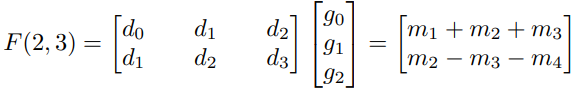
\includegraphics[width=0.8\linewidth]{images/winograd1.PNG}
	\end{center}
	\label{fig:winograd1}
\end{figure}

\begin{figure}[ht]
	\begin{center}
		% \fbox{\rule{0pt}{2in}\rule{0.9\linewidth}{0pt}}
		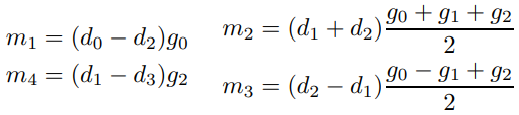
\includegraphics[width=0.8\linewidth]{images/winograd2.PNG}
	\end{center}
	\label{fig:winograd2}
\end{figure}

Using this method the 6 MULs from original convolution can be reduced to just 4 MULs. Generalizing this to two-dimensional kernels and inputs in the spacial dimension, channels and multiple filters, the arithmetic complexity can still be reduced up to a factor of 4 compared to direct convolution. This optimization is based on reducing the amount of duplication when applying kernels using a sliding window approach. It reduces the amount of computation by reducing duplication and is therefore also much more cache-efficient. \cite{AndrewLavin.2015}

%-------------------------------------------------------------------------

% Approach
\section{Approach} \label{approach}
% Explanatory figures

\subsection{Structural re-parameterization method}

Though the goal of RepVGG is to provide a plain VGG-like CNN architecture, training such an architecture with reasonable depth until convergence is hard. The degradation problem leads to an increase of the training loss curve as deeper layers struggle to learn an implicit identity function once shallower layers have learned an ideal mapping \cite{KaimingHe.2015}. Also, very deep plain CNNs make backpropagation difficult as gradients vanish when trying to reach shallower layers. Even if there had been studies to make such plain CNNs converge \cite{LechaoXiao.2018, OyebadeKOyedotun.2020}, speed-accuracy trade-off for plain CNNs remained an open research topic. To avoid the struggles to train a plain CNN directly, RepVGG uses a structural re-parameterization method to transfer model parameters from a trained ResNet-like architecture to a plain VGG-like architecture that is used for inference. 

\begin{figure}[t]
	\begin{center}
		% \fbox{\rule{0pt}{2in}\rule{0.9\linewidth}{0pt}}
		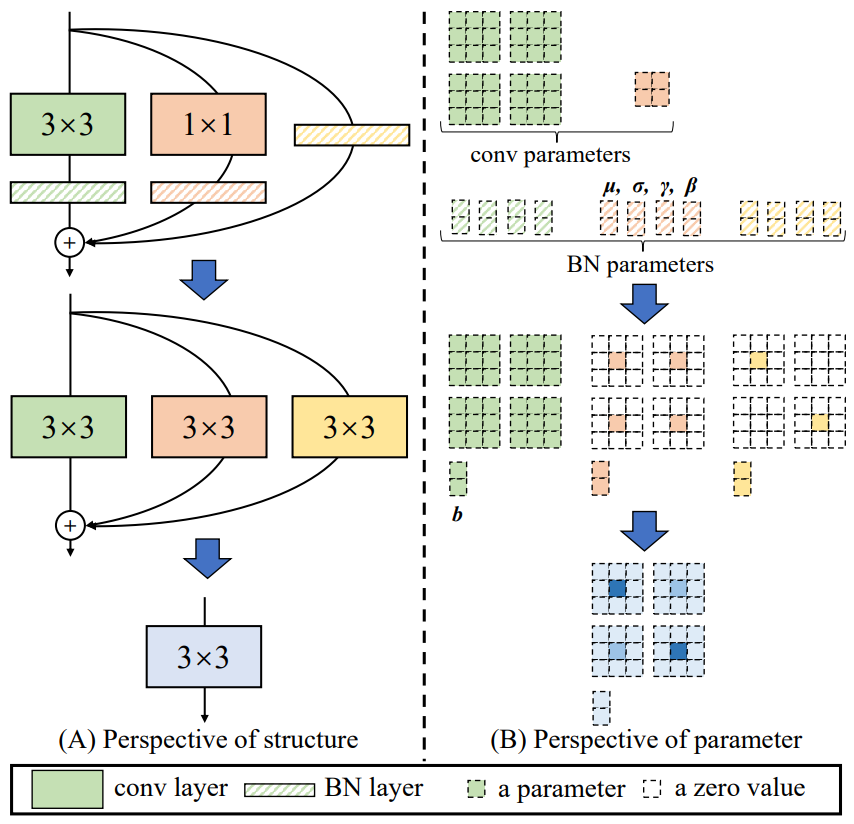
\includegraphics[width=\linewidth]{images/re-parameterization.PNG}
	\end{center}
	\caption{Structural re-parameterization method of RepVGG transforming a 3x3 convolutional layer, a 1x1 convolutional layer and an identity branch to a single 3x3 convolutional layer branch \cite{XiaohanDing.2021}.}
	\label{fig:reparameterization}
\end{figure}

One layer in the training-time architecture contains three branches, a 3x3 convolution, a 1x1 convolution and an identity branch (see \autoref{fig:reparameterization}). Having the identity branch makes the architecture ResNet-like and prevents the degradation and vanishing gradient problem. The additional 1x1 convolution branch is needed for dimensionality control in case the dimensions would not match when adding the identity shortcut connection with the 3x3 convolution branch. In this case the identity branch is omitted. Having such three branches makes the training time model an implicit ensemble of $3^n$ models with $n$ being the number of layers used. 

To transform this layer configuration to a single-path 3x3 convolution simple linear algebra is used. First the identity branch is transformed to a 1x1 convolution using the identity matrix as a kernel. The two 1x1 convolutional layers are then zero-padded to become 3x3 convolutional layers. Next the batch normalization layers need to be transformed. Batch normalization is originally applied channel-wise to every pixel in a feature map resulting from a convolutional operation of the input channel $M$ with the filter $W$ according to 

\begin{equation} \label{eq:batchnormalization}
	bn(M*W, \mu, \sigma, \gamma, \beta) = (M*W - \mu)\frac{\gamma}{\sigma} + \beta
\end{equation}

with $\mu$ being the accumulated mean, $\sigma$ being the standard deviation, $\gamma$ being the learned scaling factor and $\beta$ being the bias value. One could also realize batch normalization by adapting the convolutional filter and adding a bias value after convolution like 

\begin{equation} \label{eq:batchnormalizationtransformed}
	bn(M*W, \mu, \sigma, \gamma, \beta) = M*(\frac{\gamma}{\sigma}W) - (\frac{\mu\gamma}{\sigma} + \beta).
\end{equation}

To receive the final 3x3 convolutional layer one simply has to add all 3 kernels together as well as all 3 bias values (see \autoref{fig:reparameterization}). Note that equal striding and compatible padding configuration over the 3x3 and 1x1 branch for the image dimension is necessary to perform such re-parameterization technique (padding one pixel less for 1x1 convolution). 

\subsection{Resulting architecture}

\setlength{\tabcolsep}{5pt}
\begin{table}
	\begin{center}
		\begin{tabular}{c|c|l|l} 
			\hline
			Stage & Output size & RepVGG-A & RepVGG-B \\
			\hline
			1 & 112 x 112 & 1 x min(64,64a) & 1 x min(64,64a) \\
			2 & 56 x 56 & 2 x 64a & 4 x 64a \\
			3 & 28 x 28 & 4 x 128a & 6 x 128a \\
			4 & 14 x 14 & 14 x 256a & 16 x 256a \\
			5 & 7 x 7 & 1 x 512b & 1 x 512b \\
			\hline
		\end{tabular}
	\end{center}
	\caption{General purpose RepVGG archetype \cite{XiaohanDing.2021}.}
	\label{tab:architecture}
\end{table}
\setlength{\tabcolsep}{6pt}

Inspired by VGG \cite{KarenSimonyan.2014} and ResNet \cite{KaimingHe.2015} the archetype of RepVGG networks results in the general-purpose template shown in \autoref{tab:architecture}. Every architecture is divided into five stages where each stage downsamples by using a stride of 2 in the first layer instead of using max-pooling layers as opposed to the original VGG model. This means more hardware-optimized 3x3 convolutional layers can potentially be integrated onto the chip. To speed up inference the first stage only uses a single layer to quickly downsample high-resolution images. Most of the convolutional work is done on a small 28x28 image size in stage four following ResNet \cite{KaimingHe.2015} and RegNet \cite{IlijaRadosavovic.2020} architectural designs. With these considerations RepVGG-A and RepVGG-B were specified, the former to perform against light- and middleweight models, the latter to perform against heavyweight models. Both can be further adapted by choosing the width scaling factors $a$ and $b$ accordingly. Note that $b$ is usually chosen higher than $a$ to receive richer features. Also maximally 64 filters should be learned in stage 1 to keep computational effort for convoluting with high-resolution images limited. The scaling factor $a$ reaches from 0.75 in RepVGG-A0 to 3 in RepVGG-B3 whereas scaling factor $b$ lies between 2.5 in RepVGG-A0 to 5 in RepVGG-B3. Note that the task-specific heads still need to be added in order to complete the architecture. Therefore global average pooling and a fully-connected layer will be appended for image classification which is not shown in \autoref{tab:architecture}. 

Futher offsprings of the general-purpose RepVGG archetype use groupwise 3x3 convolution in order to make inference faster at the cost of lower accuracy. Normally such groupwise convolutional layers would implicitly increase MAC as more channels can be used within a certain FLOP constraint, but as the output channel configuration remains the same, the MAC also stays constant. Therefore instead of using dense convolution between all channels, convolution is applied groupwise in groups of 2 or 4 making convolution more sparse and therefore faster. In order to not lose inter-channel correlations throughout the network, groupwise convolution is only applied to every second layer starting from layer 3.  


%-------------------------------------------------------------------------

% Experiments and results
\section{Experiments} \label{experiments}

\subsection{Training configuration}

Not that weight initialization was not onsidered anymore here. 

\subsection{Comparison to baselines}

\begin{figure}[t]
	\begin{center}
		% \fbox{\rule{0pt}{2in}\rule{0.9\linewidth}{0pt}}
		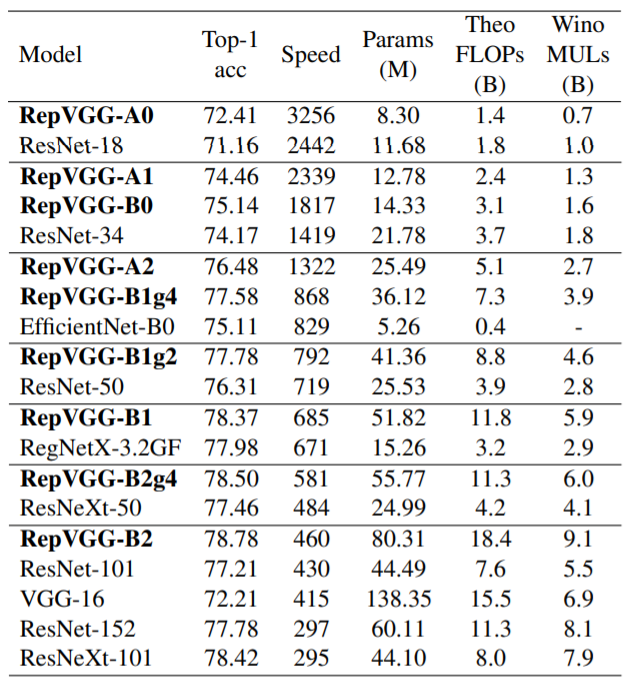
\includegraphics[width=0.8\linewidth]{images/results1.PNG}
	\end{center}
	\caption{RepVGG performance on ImageNet \cite{JiaDeng.2009} after being trained 120 epochs with simple data augmentation. The speed is measured in examples/second.}
	\label{fig:results1}
\end{figure}

When analyzing the empirical results (see \autoref{fig:results1}) one recognizes the following achievements. 

First the light- and middleweight models of RepVGG-A slightly outperform their ResNet baselines in accuracy, but achieve far higher inference speed. For instance RepVGG-A2 having a comparable amount of parameters to ResNet-50 is only 0.17\% better in accuracy, but therefor 83\% faster. Using interleaved groupwise convolutional layers such increases in speed can further be pushed, e.g. when looking at RepVGG-B1g2 and its counterpart baseline ResNet-152. Achieving the same accuracy RepVGG-B1g2 is a whole 2.66 times faster. 

When looking at the parameter efficiency RepVGG manages to outperfom the historical ResNet and VGG competitors. While achieving the same accuracy RepVGG-B1g2 only needs 69\% of the parameters of ResNet-152. The difference is even higher when comparing RepVGG-A0 to VGG-16 which state a reduction around 94\% of the parameters needed (8.30M compared to 138.35M). Obviously such parameter efficiency gains change when comparing RepVGG to more modern architectures like EfficientNet (14.33M RevVGG-B0 vs. 5.26M EfficientNet-B0) or RegNet (15.26M RegNetX-32.GF vs 41.36M RepVGG-B1g2). As the goal of RepVGG is to gain a good speed-accuracy trade-off while using a plain architecture for inference, such parameter inefficiency are justifiable and difficult to avoid. 

Also it is worth noticing that RepVGG models can of course - at the costs of the amount of parameters needed - keep up with state-of-the-art models. The authors therefore try to make a point by comparing e.g. EfficientNet-B0 to RepVGG-A2 being 1.37\% more accurate and 59\% faster. The question remains whether this can be seen as a valid argument as EfficientNet-B0 uses far less parameters compared to Rep-VGG-A2. If one compares models with approximately equal number of parameters like ResNeXt-50 to RepVGG-A2 such accuracy guarantees will no longer outperform the state-of-the-art models (77.46 vs. 76.48). Nevertheless the speed-up factors remain the strong accomplishment of all RepVGG models (484 ResNeXt-50 vs. 1322 RepVGG-A2). The comparison of ResNeXt-50 and RepVGG-A2 is in addition a perfect proof of the thesis that speed cannot be approximated with FLOPs. If so ResNeXt-50 should have been faster in inference as having less theoretical FLOPs compared to RepVGG-A2 (4.2 vs. 5.1). Winograd multiplications on the other hand seem to work as a better metric to derive speed comparisons (4.1 ResNeXt-50 vs. 2.7 RepVGG-A2). 

\begin{figure}[t]
	\begin{center}
		% \fbox{\rule{0pt}{2in}\rule{0.9\linewidth}{0pt}}
		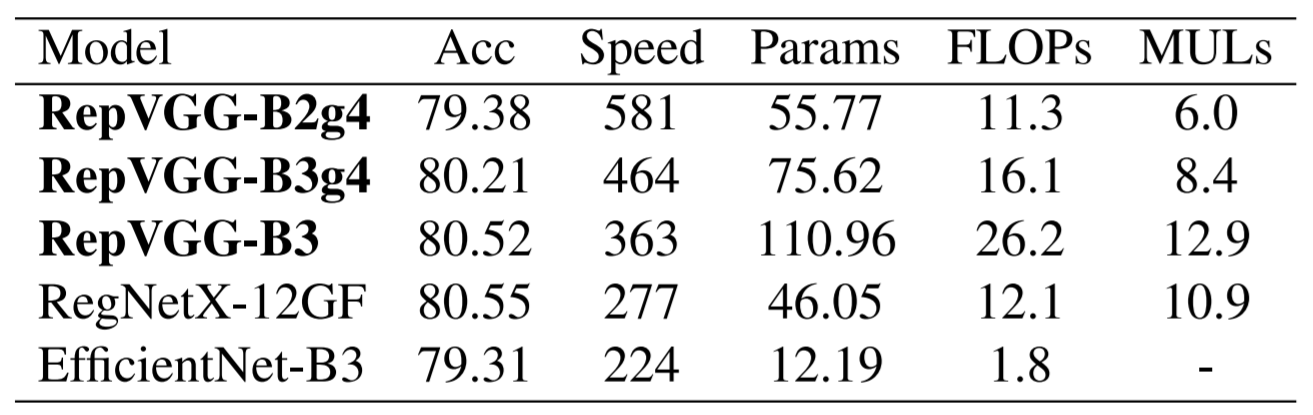
\includegraphics[width=0.8\linewidth]{images/results2.PNG}
	\end{center}
	\caption{RepVGG performance on ImageNet \cite{JiaDeng.2009} after being trained 200 epochs with Autoaugment, label smoothing and mixup.}
	\label{fig:results2}
\end{figure}

The fact that RepVGG as the first of its kind achieved an accuracy of over 80\% on ImageNet \cite{JiaDeng.2009} is also not to forget (see \autoref{fig:results2}).

\subsection{Ablation studies}

\begin{figure}[t]
	\begin{center}
		% \fbox{\rule{0pt}{2in}\rule{0.9\linewidth}{0pt}}
		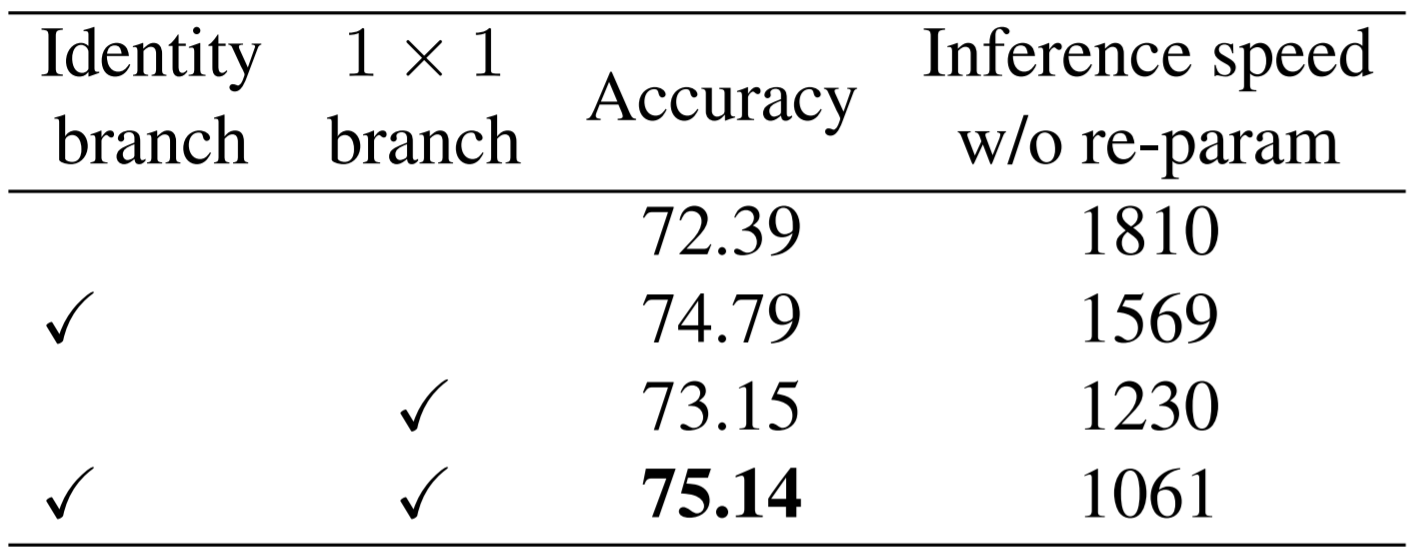
\includegraphics[width=0.8\linewidth]{images/ablation1.PNG}
	\end{center}
	\caption{Ablation studies with 120 epochs on RepVGG-B0}
	\label{fig:ablation1}
\end{figure}

In the ablation studies in \autoref{fig:ablation1} one recognizes the importance of the shortcut connections and ensemble character of RepVGG after 120 epochs of training as the performance decreases when removing the identity and/or 1x1 convolutional branches. At the same time the speed increases when switching from a multi-branch model to a single-branch model. Note that the speed is this time measured before the structural re-parameterization. 

\begin{figure}[t]
	\begin{center}
		% \fbox{\rule{0pt}{2in}\rule{0.9\linewidth}{0pt}}
		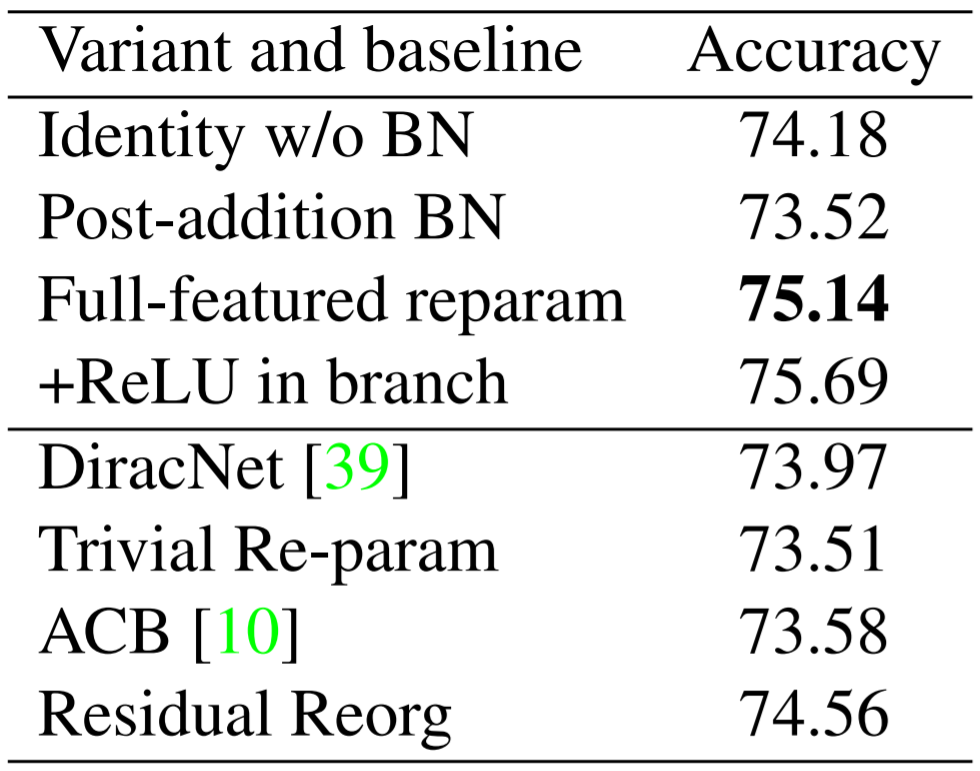
\includegraphics[width=0.8\linewidth]{images/ablation2.PNG}
	\end{center}
	\caption{Performance comparisons with architectural variants of RepVGG-B0}
	\label{fig:ablation2}
\end{figure}

The experiments shown in \autoref{fig:ablation2} are based on architectural changes of RepVGG-B0 after being trained for 120 epochs. With experiments using a DiracNet-like re-parameterization, a trivial re-parameterization (DiracNet re-parameterization with both scaling factors $a$ and $b$ set constant to 1) and another structural re-parameterization method with asymmetric convolutional blocks, interesting experiments and comparisons to other methods of re-parameterization are given. One can therefore conclude, that re-parameterization with parameters only simulating a ResNet-like architecture during training like DiracNet does is inferior to a real structural re-parameterization method like RepVGG uses. Also the success of RepVGG cannot be traced back to simple over-parameterization of each block during training when comparing the accuracy of an initial RepVGG-B0 model to a similar model with plugged-in ACB blocks replacing the RepVGG blocks. Both models therefore use over-parameterization during training and afterwards structural re-parameterization to build the inferecne model, still the RepVGG model yields in higher accuracy. RepVGG is specifically designed to make plain VGG-like CNNs trainable and achieves its higher accuracy compared to a ACB-enriched architecture through its ResNet-like training-time architecture. 

For the last comparison made in the experiments, a real residual network having one 3x3 convolutional layer in the first stage and two, three and eight residual blocks in stage two, three and four was build (shortcut connections just like ResNet-18/34). While having the same amount of 3x3 convolutional layers RepVGG still managed to outperform such an architecture (75.14 vs. 74.56), which is not surprising looking back at the first experiments made and keeping in mind that RepVGG can be seen as an ensemble of far more models. 

\subsection{Semantic Segmentation}


%-------------------------------------------------------------------------

% Discussion
\section{Discussion}

\subsection{Highlights}
- speed
- application in practice (semantic segmentation)

\subsection{Weaknesses}
% No global correlations because most layers in stage 4? (low res)

%-------------------------------------------------------------------------

% Own thoughts and conclusions
\section{Conclusion}

% TODO: Read through paper and check if nothing was forgotten (especially approach)
% TODO: Compare with presentation
% TODO: paper verlinken, z.B. nach jedem VGG und ResNet
% TODO: Grammarly korrektur
% TODO: nummern ausschreiben oder als Zahlen?
% TODO: Alle Bilder, alles und jeden zitieren (auch das RepVGG paper)
% TODO: Cite ImageNet

{\small
\bibliographystyle{ieee_fullname}
\bibliography{egbib}
}

\end{document}
